\textbf{\textsc{Exercice 4 \hfill 4 points}}

\medskip

		Sur un télésiège de la station de ski, on peut lire les informations suivantes :
		
		\begin{center}
			\renewcommand{\arraystretch}{1.2}
			\begin{tabular}{|p{5cm} p{5cm}|} \hline
					\multicolumn{2}{|c|}{\textbf{Télésiège 6 places}} \\
					Vitesse : $5,5 ~\mathrm{m}\cdot \mathrm{s}^{-1}$ & Puissance : 690 kW \\
					\multicolumn{2}{|l|}{Débit maxi : $\np{3000}$ skieurs par heure} \\
					Altitude du départ : $\np{1839}$ m& Altitude de l'arrivée : $\np{2261}$ m\\
					\multicolumn{2}{|l|}{Distance parcourue entre le départ et l'arrivée : $\np{1453}$ m} \\
					\multicolumn{2}{|c|}{ 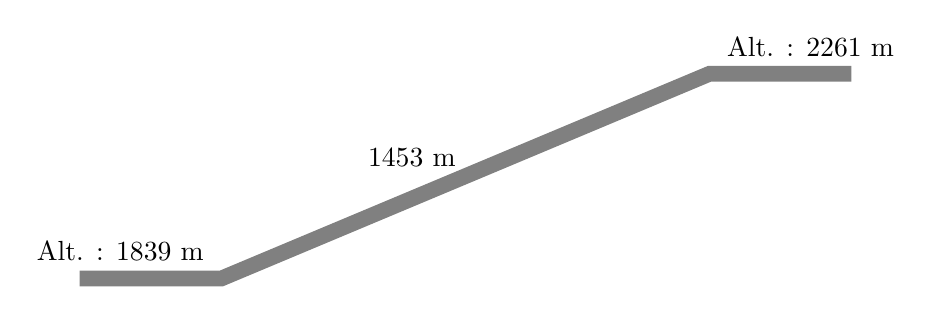
\begin{tikzpicture}[x=1.0cm,y=1.0cm] 
						\draw [line width = 2mm, color = gray] (0.,0.)-- (1.8,0.) -- (8.,2.6)-- (9.8,2.6);
						\draw (1.7,0.1) node [above left] {Alt. : $\np{1839}$ m};
						\draw (8.1,2.7) node [above right] {Alt. : $\np{2261}$ m};
						\draw (4.9,1.3) node [above left] {$\np{1453}$ m};
						\end{tikzpicture} 	} \\
					Ouverture du télésiège : 9h & Fermeture : 16h \\ \hline	
			\end{tabular}
		\end{center}
		
		\begin{enumerate}
			\item Une journée de vacances d'hiver, ce télésiège fonctionne avec son débit maximum pendant toute sa durée d'ouverture.
			
			Combien de skieurs peuvent prendre ce télésiège ?
			
			\item Calculer la durée du trajet d'un skieur qui prend ce télésiège.
			
			On arrondira le résultat à la seconde, puis on l'exprimera en minutes et secondes.
			
			\item Calculer l'angle formé avec l'horizontale par le câble de ce télésiège. On arrondira le résultat au degré.
		\end{enumerate}
		
\vspace{0,5cm}

